\chapter{Company Overview}

Rakuten is a global technology conglomerate founded in 1997 by Hiroshi Mikitani in Tokyo, Japan. Originally established under the name “MDM, Inc.”, the company was renamed Rakuten in 1999, a Japanese term meaning “optimism.” Mikitani’s vision was to build an e-commerce platform that would simplify transactions between small and medium-sized businesses and consumers. The same year, Rakuten launched Rakuten Ichiba, its flagship online marketplace, enabling merchants to create their own online stores and offer a wide variety of products ranging from clothing and electronics to everyday consumer goods.

Over time, Rakuten has significantly diversified its activities and expanded into multiple strategic sectors, including e-commerce, digital content, fintech, and telecommunications. Today, it stands as a major global player in the digital economy, leveraging innovation, data, and technology to deliver a wide ecosystem of services.

\section{Rakuten Group}

Rakuten has evolved into a diversified global group operating across several major industries.

In e-commerce, its marketplace platforms connect merchants worldwide with international consumers, offering a broad range of products and services.

In digital content, Rakuten provides services such as Kobo, a digital book platform offering over 56 million titles, as well as Rakuten Viki and Rakuten TV, which deliver ad-supported video streaming services (AVOD). The company also operates Rakuten Music, an unlimited music streaming service.

In the fintech sector, Rakuten offers a wide range of financial services including credit cards, online brokerage, banking, insurance, and its loyalty ecosystem powered by Rakuten Points. It is also a leading player in online payments and the largest credit card issuer in Japan.

In telecommunications, Rakuten owns Viber, a globally ranked instant messaging application, and operates Rakuten Mobile, the fourth-largest mobile network operator in Japan.

\noindent
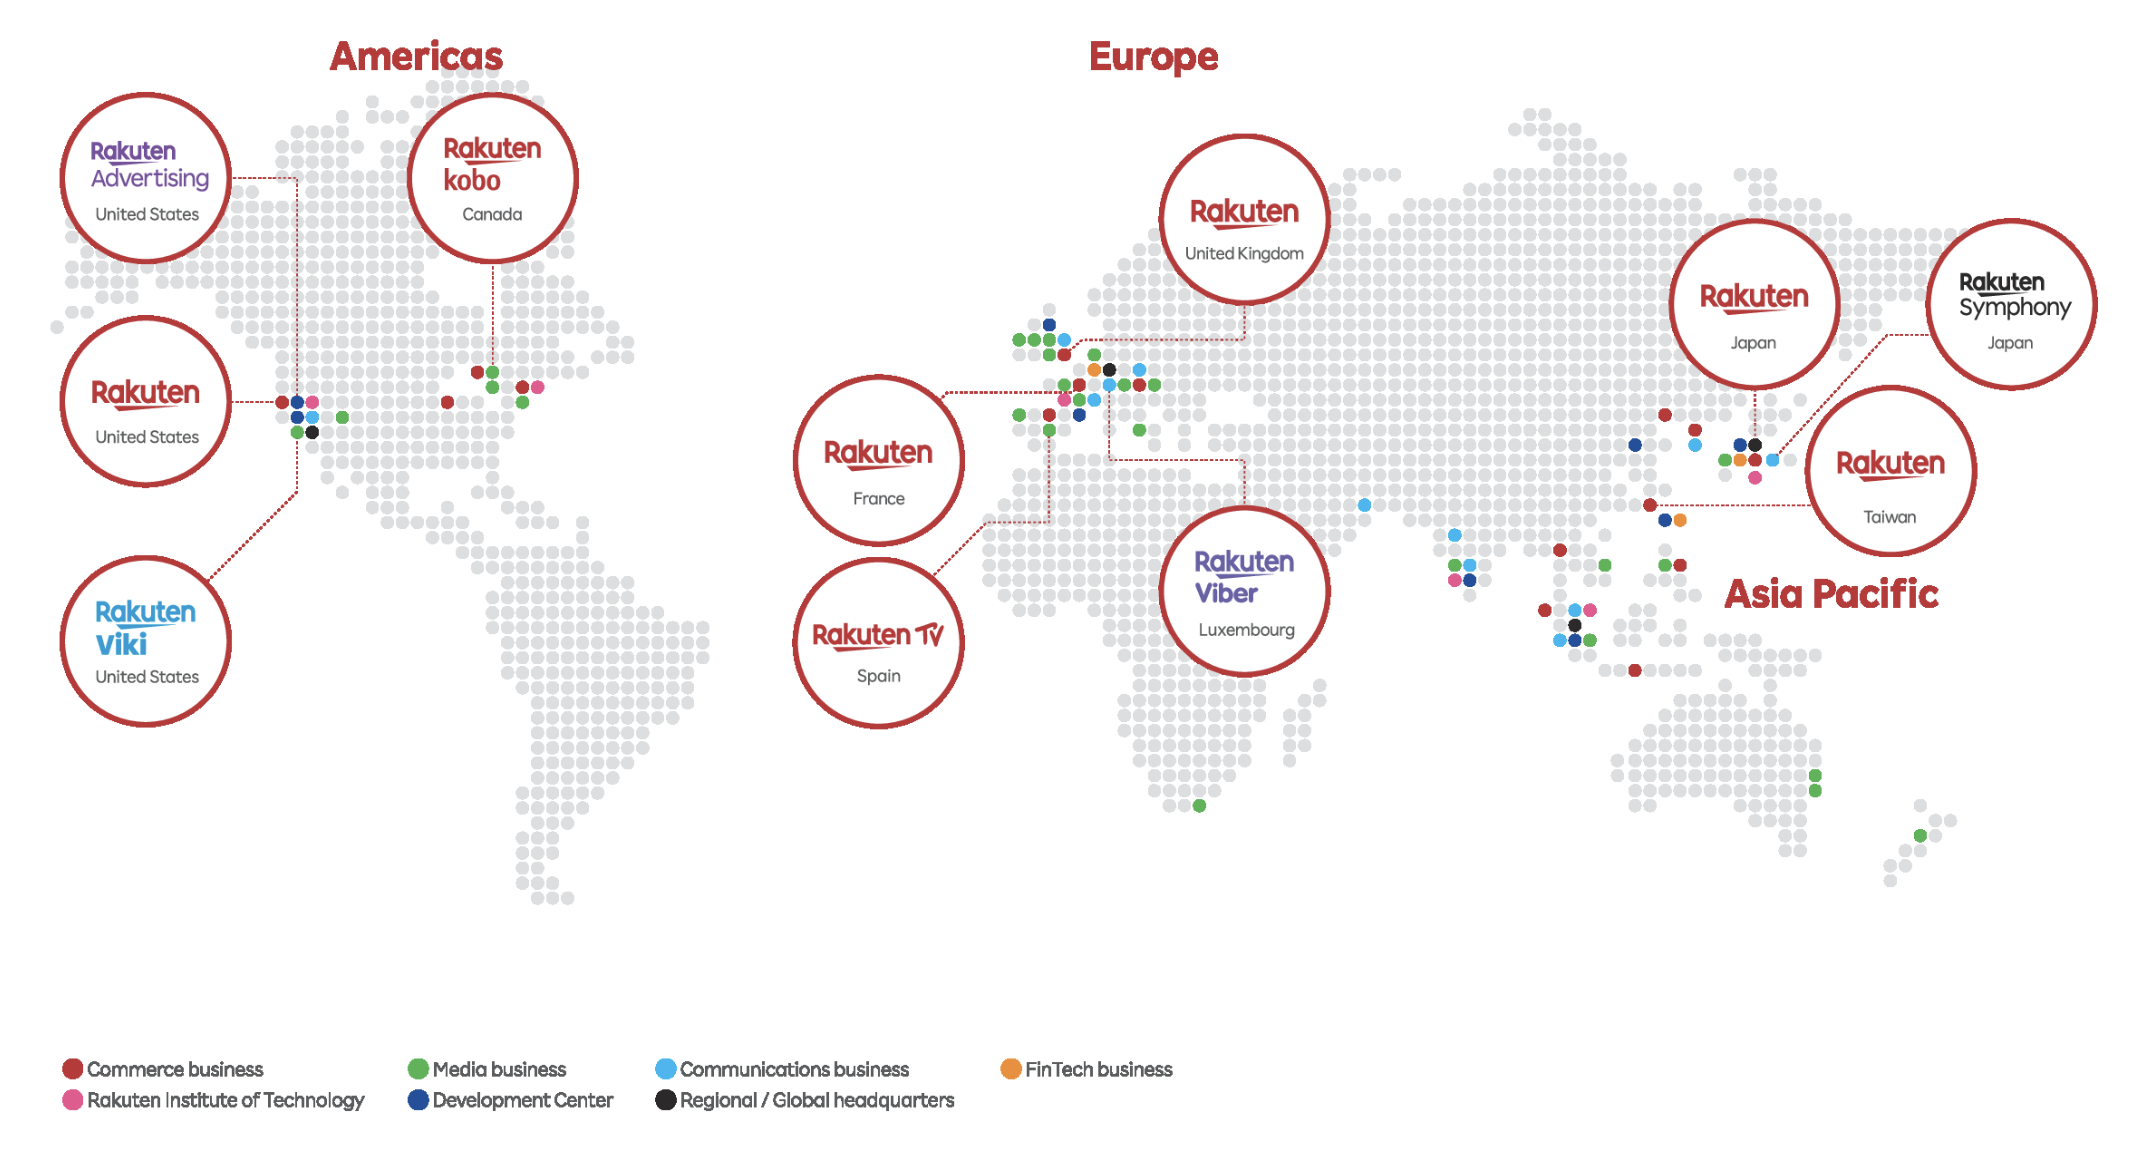
\includegraphics[width=\textwidth]{../assets/rakuten/rakuten_international.png}

\section{Rakuten France}

Rakuten France, formerly known as PriceMinister (founded in 2000), is a leading French e-commerce platform acquired by Rakuten in 2010. It connects thousands of merchants with consumers and offers a wide range of products, from cultural goods to electronics and fashion.

The company places strong emphasis on customer satisfaction, community trust, and engagement, while actively participating in sustainability and corporate social responsibility initiatives. Through continuous investment in technology and innovation—particularly in artificial intelligence and big data analytics—Rakuten France has strengthened its position as a key player in the French e-commerce market, recognized for its reliability and service quality.

\noindent
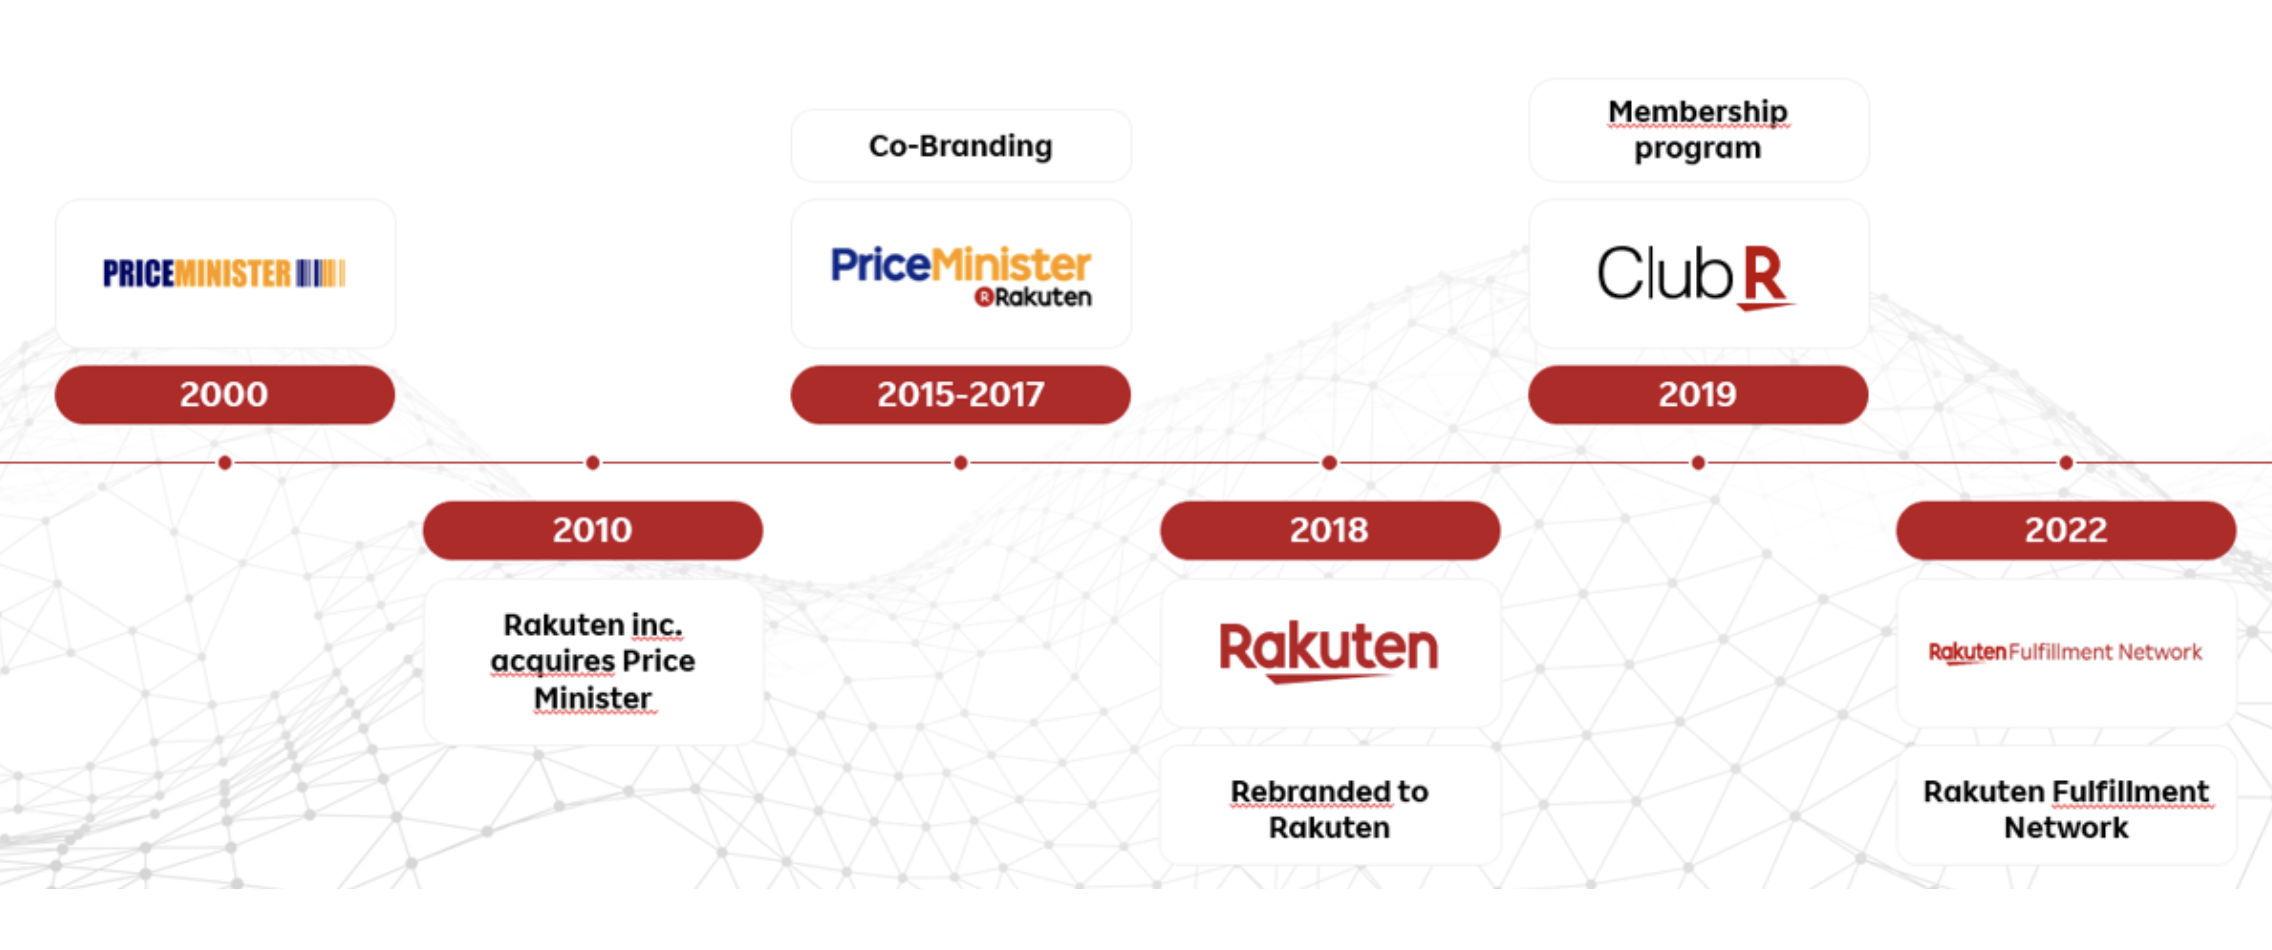
\includegraphics[width=\textwidth]{../assets/rakuten/price_minister_to_rakuten_france.png}